\documentclass[border=4pt]{standalone}
\usepackage{tikz}
\usetikzlibrary{arrows.meta}
\begin{document}
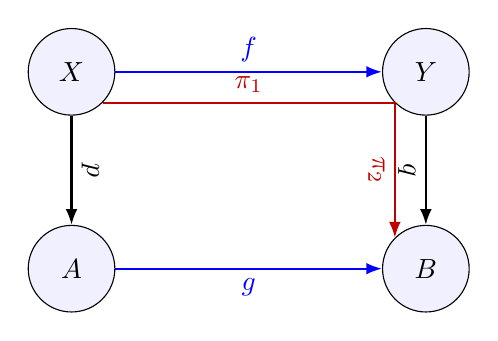
\begin{tikzpicture}[
  auto,
  object/.style={draw,circle,minimum size=11mm,fill=blue!6},
  morphism/.style={-{Latex[length=2mm]},thick}
]
  \node[object] (X) at (0,2.5) {$X$};
  \node[object] (Y) at (4.5,2.5) {$Y$};
  \node[object] (A) at (0,0) {$A$};
  \node[object] (B) at (4.5,0) {$B$};

  \draw[morphism,blue] (X) -- node[sloped] {$f$} (Y);
  \draw[morphism,blue] (A) -- node[sloped,swap] {$g$} (B);
  \draw[morphism] (X) -- node[sloped] {$p$} (A);
  \draw[morphism] (Y) -- node[sloped,swap] {$q$} (B);
  \draw[morphism,red!75!black] (X.south east) -|
    node[pos=.25,sloped] {$\pi_1$}
    node[pos=.75,sloped,swap] {$\pi_2$}
    (B.north west);
\end{tikzpicture}
\end{document}
